\documentclass[11pt]{article}
\usepackage{amsmath}

\setlength{\textwidth}{6.2in}
\setlength{\oddsidemargin}{0.3in}
\setlength{\evensidemargin}{0in}
\setlength{\textheight}{8.7in}
\setlength{\voffset}{-.7in}
\setlength{\headsep}{26pt}
\setlength{\parindent}{10pt}
\usepackage{amsfonts} % if you want blackboard bold symbols e.g. for real numbers
\usepackage{graphicx} % if you want to include jpeg or pdf pictures
\usepackage{graphics}
\usepackage{breqn}
%\usepackage{mcode}
%\usepackage{epstopdf}
\usepackage{float}
\usepackage{tabularx}
\usepackage{lscape}
\usepackage{adjustbox}
\begin{document}

%\input{exermacros.tex}       % more macros for exercise formatting
% header:
\begin{center}
{\Large \bf Answers - Machine Learning: Stock returns prediction}
\end{center}

%%%%%%%%%%%%%%%%%%%%%%%%%%%%%%%%%%%%%%%%%%%%%%%%%%%%%%%%%%%%%%%%%%%%%%%%%%%%%%%%%%%%%%%%%%%%%%%%%%%%%%%%%%%%%%%%%%%%%%%%%%%%%%%%%%%%%%%
\section{Which variables matter for predicting \(S1\)?}
The top 4 predictors of \(S1\) are {\bf \(S5, S9, S3\)} and {\bf \(S7\)}.  An uni-variate feature scoring routine with split-shuffle cross validation using regularized linear regression on the training data is employed. The mean {\(R^{2}\) scores from the cross validation samples are then used to identify the top features. The correlation between the top features are not taken into account at this stage. The figure below shows the strength of each predictor variable individually in predicting \(S1\). 
\begin{figure}[H]
\caption{Univariate Feature Scoring using \(R^{2}\)}
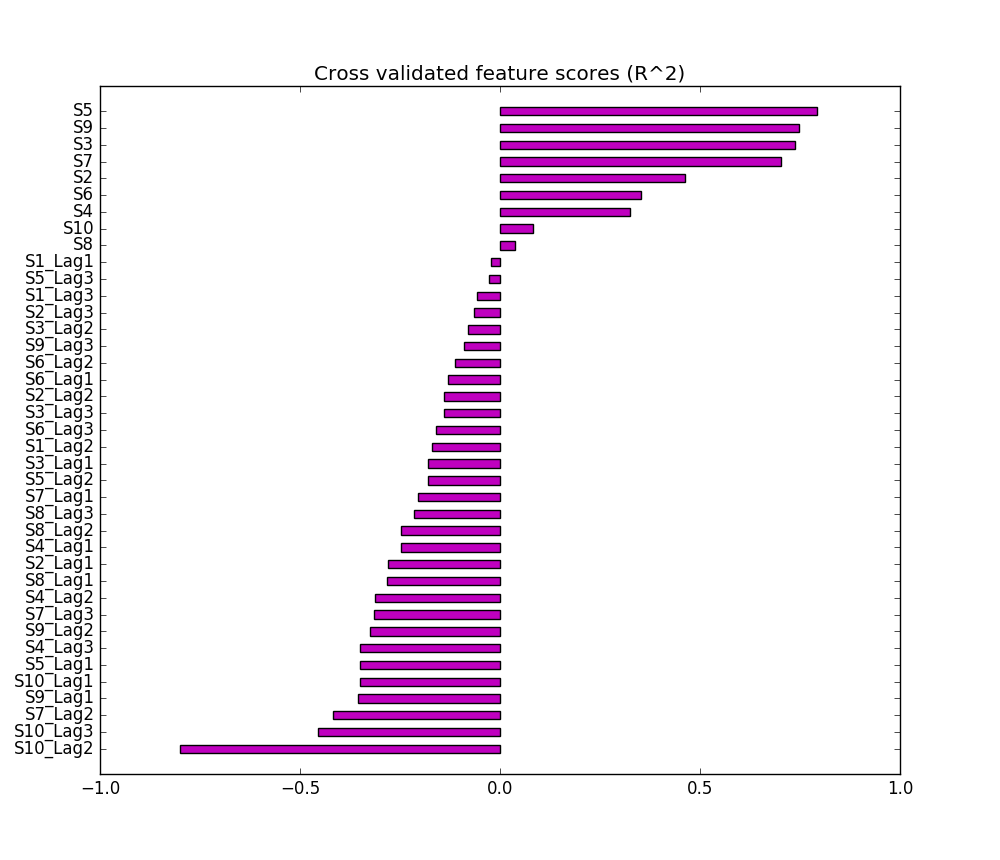
\includegraphics[width=1\textwidth,center]{fig1.png}
\end{figure}

\section{Does \(S1\) goes up or down over this period?}
\(S1\) does goes up. The model predicts a gain of approximately \(5\%\) in stock price over the entire duration.

\section{How much confidence you have in your model, when and why will it fail?} \\ 
The model yielded an average coefficient of determination of \(0.88\) on the test data. The major assumption of this model is that the Japanese stocks are highly correlated to the US stock market. Therefore, the model could fail when there is a disruption in the trends between the Japanese and American stock markets or any seasonality effects that could be related to only one market. Also, since the model is heavily dependent on the \(4\) stocks that are highly correlated to \(S1\), any internal events in the companies to which the top predictors belong to could lead to poor performance of the model.

\section{What techniques did you use and why?}
\subsection{Preprocessing}
The data is split into two sets. The model data of 50 samples was split into \(25\%\) test data and the remaining was assigned to training data. In addition to the direct predictors \((S2,S3..S10)\), lagged features for each of the predictors along with the lagged returns of the stock that is predicted \((S1\) are included in the features list. A lag of \(3\) was selected and this resulted in the total number of features to be \(9 \;  + \; 3 \* 10 = 39\). Additional features were not considered as the number of samples available is limited and the \(S1\) did not show any complex or unique trends in comparison to the predictor stocks.


\subsection{Method selection}
Regularized linear regression was selected as the feature ranking process revealed features that are highly correlated to the estimated variable \(S1\). Regression also helps to interpret the relationships between \(S1\) and the other stocks easily than other sophisticated algorithms. Another reason for selecting regression is due to the small number of data points available to model. \(L_{2}\) Regularization was selected to avoid over-fitting and to yield a more robust model for forecasting prices.

\subsection{Parameter selection}
The regularization parameter \(\alpha\) is selected by using a cross validation routine that searches for the best alpha on the training data. \(RidgeCV\) module from sklearn with \(5-\)fold cross validation was employed.

\subsection{Feature selection}
After selecting the parameter, the unimportant features are eliminated by using the recursive feature selection method. Initially, a recursive feature selection with cross-validation module \(RFECV\) was used to determine the number of features required for the best fit on different iterations of cross-validation. Multiple cross-validation strategies were used and the mean number of features selected was \(5\), which is consistent with the number of top features estimated in the feature ranking process. However, since our training data is small, a more conservative model, with \(8\) features was selected for increased robustness using the \(RFE\) module. This module selects the best \(8\) features on the training data and this included the lag variables of \(S_1\) returns, indicating auto-correlation, which was expected in time series data.

\subsection{Test score}
Finally, the model was used to predict \(S1\) for the test data that was initially withheld and the coefficient of determination returned was 0.88. I think even for the worst case scenario, this model should have a prediction accuracy of ~ \( 80\% \).

\end{document}
